\documentclass{scrartcl}

\usepackage[ngerman]{babel}
\usepackage{fontspec}

% some useful packages
\usepackage{mathtools}
\usepackage{amssymb}
\usepackage{graphicx}
\usepackage[printwatermark]{xwatermark}
%\usepackage{hyperref}
%wird eh durch error durch default ersetzt -> auskommeentiert
%\hypersetup{%
%	pdfborder={0 0 0}
%}
\usepackage{titlesec}

\newwatermark*[pages=16-20,color=gray!75,angle=45,scale=3,xpos=0,ypos=0]{DRAFT}
\newcommand{\sectionbreak}{\clearpage}

\usepackage{ifthen}

\newenvironment{requirements}{
	\begin{itemize}
}{
	\end{itemize}
}

\newcommand{\req}[2][]{
	\item[/#2/]\label{#2}\ifthenelse{\equal{#1}{}}{}{ \textbf{#1}}
}

\newcommand{\itm}[1]{\item{\texttt{#1}}}


\setmainfont{SourceSerifPro-Regular.otf}[
    BoldFont    = SourceSerifPro-Bold.otf
    ItalicFont  = EBGaramond08-Italic.otf
]

\begin{document}
\setlength{\parindent}{0pt}

\begin{titlepage}

%Title
\begin{center}
	\huge \bfseries Chrono Command \\
	\large  Web Basierte Zeiterfassung
\end{center}

%Subtitle
\begin{center}
	\large Pflichtenheft \\
\end{center}

%Authors
\begin{center}
	Jannis Friedmann \\
	David Kuhmann \\
	Maria Schmid \\
	Xiaoming Wang \\
	Jan Zenkner \\

\end{center}

%Date
\begin{center}
	\large \today
\end{center}
	
\vfill

\iffalse
\title{Pflichtenheft}
\author{ 
	Jannis Friedman\and
	David Kuhmann\and
	Maria Schmidt\and
	Xiaoming Wang\and
	Jan Zenkner
}
\date{\today}
\end{titlepage}
\maketitle
\thispagestyle{empty}

\fi
\pagenumbering{roman}

\clearpage
\pagestyle{empty}
\tableofcontents

\clearpage
\pagestyle{plain}
\pagenumbering{arabic}
\setcounter{page}{1}

\section{Einleitung}

Auf herkömmlicher Weise muss ein \emp{Benutzer*} (Studenten*) seinen \emp{Stundenzettel} monatlich manuell erstellen und an seinen \emph{Betreuer*} übergeben. Nach einer erfolgreichen Kontrolle muss der \emph{Betreuer*} den \emph{Stundenzettel} an das Sekretariat zur Bearbeitung weiterleiten. \\

Es können an einer Universität hunderte bis tausende Stundenten* beschäftigt sein. Diese manuellen Vorgänge sind extrem zeitaufwändig und außerdem könnten viele Fehler sowie Probleme dabei auftreten.\\

Das Ziel des Projekts ist, ein professionelles und komfortables Zeiterfassungssystem als Web Front-end zu entwickeln, mit dem die \emph{Stundenzettel} von Arbeitern* an Universitäten digital statt manuell erfasst werden können und die Verwaltungsarbeiten von \emph{Betreuern*} und \emph{Administratoren*} erleichternt werden können.\\

Mit diesem digitalen Zeiterfassungssystem sollen folgende Vorteile erreicht werden:\\

\begin{itemize}
	\item Durch die automatische Datenübernahme wird der manuelle Aufwand auf ein Minimum reduziert, das heißt Zeit- und Kostenersparnis.
	\item verhindert Verletzungen der Vorgabe des Gesetzes, z.B. Arbeiten an Feiertagen, Arbeiten über Gesetzlimit usw.
	\item effiziente Projektverwaltung durch die getrennte Erfassung verschiedener Tätigkeiten.
	\item übersichtlichere Verwaltung durch grafische und tabellarische Darstellung
\end{itemize}

\section{Zielbestimmung}

\subsection{Musskriterien}

\begin{itemize}
	\item Starten und Stoppen von einer Zeiterfassung
	\item Zeiten sind nachträglich erfassbar
	\item erfasste Zeiten sind können Tätigkeiten zugeordnet werden
	\item Warnungen wenn Zeiten nicht eingetragen
	\item Möglichkeit die erfassten Zeiten an den Admin zu übersenden
	\item Warnungen wenn gesetzlich Pausen genommen werden müssen
	\item Vergangene Zeiten einsehbar
	\item Hinzufügen von Accounts
	\item Löschen von Accounts
	\item Ändern von Accounts
	\item Bestimmte Benutzer sind Administratoren
	\item Bestimmte Benutzer sind Betreuer
	\item Administratoren legen fest welche Benutzer von welchem Betreuer betreut werden
	\item Backups werden regelmäßig angefertigt
	\item Es kann zwischen LDAP und lokalen Accounts zur Benutzerverwaltung gewählt werden
\end{itemize}


\subsection{Wunschkriterien}

\begin{itemize}
	\item Mehrere Frontendimplementierungen sind möglich
	\item Zeitvorhersagen anhand vergangener Arbeitszeit
	\item Überwachung der Arbeitszeit auch ohne abgebene Zeiten möglich
	\item Zeiten sollen durch eine graphische Übersicht visulisiert werden
	\item Erfassung der Tätigkeiten während der Arbeitszeit

\end{itemize}


\subsection{Abgrenzungskriterien}
\begin{itemize}
	\item Korrekter Ablauf im Internet Explorer wird nicht unterstüzt
\end{itemize}

\section{Produkteinsatz}
Das System dient zur Verwaltung und Kontrolle der Arbeitszeiten von Mitarbeiter (Studenten), Analyse verschiedener Projekte anhand der erfassten Zeiten und der entsprechenden Tätigkeiten. Die von Benutzern angegebenen Daten werden auf einem Server gespeichert. Auf dem Server gespeicherte Daten können mit einem Internet Browser aufgerufen, tabellarisch und grafisch dargestellt werden. Durch Nachrichtenfunktionen soll der Kontakt zwischen Benutzern, Betreuern und Admin sichergestellt werden. Des Weiteren gibt es eine Benutzerverwaltung, um die Zugriffsrechte auf die Daten zu verwalten.
\subsection{Anwendungsbereiche}
\begin{itemize}
	\item Der Anwendungsbereich umfasst sämtliche gewerbliche Betriebsumfelder sowie Universitäten, Institutionen, Vereine, welche die Arbeitszeiten von HIWIs oder ähnlichen Mitarbeitern auf effizienter Weise verwalten wollen. Die Anzahl der Studenten bzw. Mitarbeitern sind normalerweise groß.
\end{itemize}

\subsection{Zielgruppen}
\begin{itemize}
	\item Die Anwender in den Zielgruppen sind Benutzer, Betreuer und Administrator. Die Zielgruppen haben ein gruppeneigenes Berechtigungsprofil, das auf die Benutzerbedürfnisse zugeschnitten ist und nur Zugriff auf die nötigen Funktionen erlaubt. Dabei hat der Benutzer nur Zugriffsberechtigung auf seine eigenen Daten, während der Betreuer auf alle seinen zugewiesenen Benutzer und der Administrator auf alle Daten Zugriff hat.
\end{itemize}

\subsection{Betriebsbedingungen}
\begin{itemize}
	\item Die Betriebsbedingungen müssen für die Anwendung auf einem zentralen Webserver spezifiziert werden. Der Server läuft im Dauerbetrieb und unbeaufsichtigt. Client-User brauchen einen normalen Internetfähigen Rechner oder Smartphone.
\end{itemize}

\section{Produktumgebung}

\subsection{Software}
\subsubsection{Software Backend}
\begin{itemize}
    \item Als Basis des \em{Backends} dient Java 8.
    \item Das Erstellen der benötigten Dateien übernimmt Maven.
    \item Als Interface für die \em{Datenbank} wird Hibernate ORM genutzt.
            Zur Datenbankanbindung wird dabei JDBC genutzt.
    \item Für die Authentifikation wird Apache Shiro verwendet.
    \item Das Generieren der PDF-Dateien aus den \em{Stundenzetteln} wird mithilfe von Apache PDFBox realisiert.
\end{itemize}

\subsubsection{Software Frontend}
\begin{itemize}
    \item Das \em{Frontend} ist eine auf HTML5 basierte Weboberfläche und wird mithilfe von VAADIN aus Java Code generiert.
\end{itemize}

\subsection{Hardware}
\subsubsection{Hardware User}
\begin{itemize}
    \item Da die Anwendung auf einer Web-Oberfläche läuft ist, muss die Hardware einen Webbrowser besitzen der HTML5 und JavaScript unterstützt.
\end{itemize}

\subsubsection{Hardware Server}
\begin{itemize}
    \item Der Server muss Java 8 installiert haben.
    \item Es wird ein Java Servlet Webserver benötigt.
    \item Es muss eine JDBC-kompatible Datenbank vorhanden sein.
\end{itemize}

\section{Funktionale Anforderungen}

Die den Wunschkriterien zugeordneten Anforderungen sind mit einem "`+"' hinter der Indentifikationsnummer markiert.

\subsection{Stundenzettel und Zeiterfassung}

\begin{requirements}
    \req[Zeiterfassung]{F110}
    Ein User kann in seiner Hauptseite eine Zeiterfassung starten und stoppen.
    \begin{requirements}
        \req[Kategorie]{F111} Eine Zeiterfassung ist mit einer Kategorie versehen.
        \req[Tätigkeit]{F112} Eine Zeiterfassung ist mit einer Tätigkeit verbunden.
        \req[Zeiterfassung ändern]{F113} Eine Zeiterfassung kann nachträglich geändert werden.
        \req[Alternative Zeiterfassung]{F114} Eine Zeiterfassung kann auch manuell ohne das Starten und Stoppen einer Zeit erfasst werden.
        \req[Zeiterfassung löschen]{F115} Eine erfasste Zeit kann vom Benutzer wieder gelöscht werden
    \end{requirements}

    \req[Gesetzliche Vorgaben]{F120}
    Die Zeiterfassung und der Stundenzettel folgen den gesetzlichen Bestimmungen.
    \begin{requirements}
        \req[Maximale Arbeitszeit]{F121} Die gesetzlich maximale Arbeitszeit kann bei einer Zeiterfassung nicht überschritten werden
        \req[Pausenzeiten]{F122} Eine Zeiterfassung kann nicht dem Stundenzettel hinzugefügt werden wenn für ihren Umfang gesetzliche Pausenzeiten nicht eingetragen wurden.
    \end{requirements}

    \req[Stundenzettel]{F130}
    Der Stundenzettel stellt eine Aufzeichnung der Arbeitstunden in einem vorgesetzten Zeitraum dar.
    \begin{requirements}
        \req[Sichtbarkeit]{F131} Der Betreuer und der Administrator können den Stundenzettel einsehen.
        \req[Stundenzettel abgeben]{F132} Ist der Benutzer mit seiner Zeiterfassung in einem Zeitraum fertig, so kann er den Stundenzettel abgeben.
        \req[abgegebene Stundenzettel]{F133} Der Betreuer und der Admin werden über abgegebene Stundenzettel Informiert
        \req[Stundenkonto]{F134} Im Stundenzettel ist die tatsächliche und die zu leistende Arbeitszeit sichtbar.
        \req[Betreuerkontrolle]{F135} Ein Stundenzettel kann vom Betreuer als Okay befunden werden.
        \req[Stundenzettel exportieren]{F136} Ein Administrator kann alle Stundenzettel für einen Monat zum Drucken exportieren
    \end{requirements}

\end{requirements}

\subsection{Benutzer und Rechte}

\begin{requirements}
    \req[Benutzer]{F210}
    Ein Benutzer stellt den Standart User dar.
    \begin{requirements}
        \req[Stundenzettel]{F211} Ein Benutzer kann nur seinen eigenen Stundenzettel einsehen und verändern.
        \req[Warnungen]{F212} Ein Benutzer erhält nur Warnungen über seine eigenen Aktionen.
        \req[Erinnerungen]{F213} Ein Benutzer erhält nur Erinnerungen, die ihn selbst betreffen.
    \end{requirements}

    \req[Betreuer]{F220}
        Ein Betreuer ist für mehrere Benutzer zuständig.
        \begin{requirements}
            \req[Benutzer zuweisen]{F221} Einem Betreuer können Benutzer zugewiesen werden
            \req[Stundenzettel]{F222} Der Betreuer kann über seine übersicht alle ihm zugewiesenen Benutzer einsehen
            \req[Warnungen]{F223} Der Betreuer erhält Warnungen für alle Benutzer die ihn zugewiesen sind.
            \req[Erinnerungen]{F224} Der Betreuer erhält Erinnerungen für alle Benutzer die ihm zugewiesen sind.
            \req[Stundenzettel prüfen]{F225} Der Betreuer überprüft die agegebenen Stundenzettel der im zugewiesenen Benutzer.
        \end{requirements}

    \req[Admin]{F230}
        Ein Admin stellt das Verwaltungsorgan dar.
        \begin{requirements}
            \req[Benutzer erstellen]{F231} Der Admin kann neue Benutzer anlegen.
            \req[Benutzer editieren]{F232} Der Admin kann die Daten existierende Benutzer verändern.
            \req[Benutzer löschen]{F233} Der Admin kann einen existierenden Benutzer löschen.
            \req[Benutzer zuweisen]{F234} Der Admin kann Benutzer einem Betreuer zuweisen.
            \req[Betreuer Ansicht]{F235} Der Admin kann für jedes Team auch auf die Betrueransicht zugreifen.
        \end{requirements}
\end{requirements}

\subsection{Zeitüberwachung und Darstellung}
    \begin{requirements}
        \req[Graphische Darstellung Zeit]{F310+}
        \begin{requirements}
            \req[Übersicht Teams]{F311} Der Admin soll die bisher benötigte Zeit aller Teams auf seiner Hauptseite einsehen können.
            \req[Übersicht Betreuer]{F312} Dem Betreuer soll die bisher benötigte Zeit aller im zugewiesenen Benutzer angezeigt werden.
            \req[Übersicht Benutzer]{F313} Der Benutzer soll seine bisher aufgewedete Zeit graphisch angezeigt werden.
        \end{requierements}

        \req[Graphische Darstellung Stundenzettelabgabe]{F320}
        \begin{requirements}
            \req[Übersicht Teams]{F321} Der Admin soll auf seiner Hauptseite die bisherigen Abageben von Stundenzetteln angezeigt bekommen.
            \req[Übersicht Betreuer]{F322} Der Betreuer soll den bisherigen Abgabefortschritt seines Teams dargestellt bekommen.
        \end{requirements}

        \req[Magie mit Daten]{F330}
        \begin{requirements}
            \req[Heatmap]{F331} Benutzer können einsehen an welchen Tagen die meinste Arbeitszeit geloggt wurde.
            \req[Punch Card]{F332} Benutzer können einsehen zu welchen Zeiten die meinste Arbeitszeit geloggt wurde.
        \end{requirements}

        \req[Tätigkeiten Darstellung]{F340}
        \begin{requirements}
            \req[Tätigkeiten Ranking]{F341} Benutzer können sich den Zeitverbrauch pro Tätigkeit, gesammlt über alle Benutzer, anzeigen lassen.
            \req[Tätigkeits Heatmap]{F342} Benutzer können sich eine Tätigkeits Heatmap, anzeigen lassen.
        \end{requirements}

    \end{requirements}


\section{Produktdaten}

\subsection{Benutzerdaten}
\begin{requirements}
	\req [Benutzer*] {D10}
	\begin{requirements}
		\req{D11} ID
		\req{D12} Name
		\req{D13} Vorname
		\req{D14} Email
		\req{D15} Passwort
		\req{D16} Rechte
		\req{D17} \emph{Zeiterfassungen}
		\req{D18} \emph{Betreuer}
		\req{D19} \emph{Team}
	\end{requirements}
\end{requirements}

\subsection{Zeitdaten}
\begin{requirements}
	\req [Zeiterfassung] {D20}
	\begin{requirements}
		\req{D21} \emph{Benutzer*} ID
		\req{D22} \emph{Kategorie}
		\req{D23} \emph{Tätigkeit}
		\req{D24} Beginn
		\req{D25} Ende
	\end{requirements}

	\req [Stundenzettel] {D30}
	\begin{requirements}
		\req{D31} \emph{Benutzer*} ID
		\req{D32} \emph{Zeiterfassungen}
		\req{D33} Stundenkonto
		\req{D34} Abgeschlossen
		\req{D35} \emph{Betreuer*} geprüft
	\end{requirements}
\end{requirements}



\section{Nichtfunktionale Anforderungen}

\subsection{Allgemeine Ziele}
\begin{requirements}
    \req{NF110} Die Navigation durch die Weboberfläche ist Intuitiv.
\end{requirements}

\subsection{Benutzbarkeit, Performance und Stabilität}
\begin{requirements}
    \req{NF220} Die Ladezeit des Frontends liegt bei guter Internetverbindung unter 30 Sekunden.
    \req{NF230} Es wird auf Einblendungen, die die Benutzung des Frontends einschränken verzichtet.
    \req{NF240} Das Frontend läuft stabil, das bedeutet:
     \begin{itemize}
        \item Das Frontend verhält sich zu jedem Zeitpunkt vorhersehbar.
        \item Alle Zustände und Übergänge sind zu jedem Zeitpunkt definiert
        \item unerwartete Eingaben werden abgefangen.
        \item Im Ein-Benutzer Betrieb ist das Frontend stabil (Eine Zeiterfassung pro Nutzer).
     \end{itemize}
     \req{NF250} Das Backend läuft stabil, das bedeutet:
          \begin{itemize}
             \item Das Backend verhält sich zu jedem Zeitpunkt vorhersehbar.
             \item Alle Zustände und übergänge sind zu jedem Zeitpunkt definiert
             \item unerwartete Eingaben werden abgefangen.
             \item Das Backend verhält sich in folgenden Grenzen stabil:
	\begin{itemize}
                    \item Es werden höchtens 25 gleichzeitige Anfragen an das Backend gestellt.
                \end{itemize}
          \end{itemize}
\end{requirements}

\subsection{Modularisierung in der Entwicklung}

\begin{requirements}
    \req{NF300} Um die Entwicklung und die Wartbarkeit des Produktes zu unterstützen, wird das Produkt in Module unterteilt.
    \begin{requirements}
        \req{NF310}Die Datenbank wird nicht Modularisiert.
        \req{NF320} Das Backend wird in folgende Module unterteilt:
            \begin{itemmize}
                \item TODO
            \end{itemize}
        \req{NF330} Das Frontend wird in folgende Module unterteilt:
            \begin{itemize}
                \item Zeitmessung
                \item Benachrichtigungen
                \item Kalender
                \item Statistiken
                \item Stundenzettel Kern
            \end{itemize}
    \end{requirement}
\end{requirements}

\subsection{Qualität und Rechtliches}
\begin{requirements}
    \req{N410} Die in Laufe des Projekts erstelle Artefakte sind gut
    \begin{itemize}
        \item zu warten (Einhaltung von Code Standarts).
        \item zu erweitern (Objektorientierter, modularer Aufbau.)
        \item dokumentiert.
        \item mit Testfällen abgedeckt (Unittests, Überdeckung > 75\%).
    \end{itemize}
    \req{NF420} Eine kommerzielle Veröffentlichung des Produkts ist möglich, u.a. gilt:
    \begin{itemize}
        \item benutzte Assets und Bibliotheken sind kommerziell nutzbar.
    	\item es finden sich Hinweise auf die jeweiligen Urheber und Lizenzen im Programm.
    \end{itemize}
    \req{NF430} Datenbankelemente liegen mindestens in der dritten Normalform vor.
\end{requirements}

\section{Globale Testfälle}

\subsection{Funktionssequenzen}
\begin{requirements}
	\req{T110} Benutzer Meldet sich an
	\begin{itemize}
  			\item Der Benutzer wählt in seinem Webbrowser die Website der Zeiterfassung an
  			\item Da der Benutzer keinen Session Cookie besitzt wird ihm ein Anmeldescreen gezeigt
  			\item Der Benutzer gibt dort seine Email an
  			\item Der Benutzer gibt dort sein Passwort an
  			\item Der Benutzer klickt auf die Schaltfläche "Anmelden"
  			\item Wenn Email und Passwort korrekt, hat sich der Benutzer damit erfolgreich angemeldet
	\end{itemize}
	\req{T120} Angemeldeter Benutzer startet/stoppt eine Zeiterfassung
	\begin{itemize}
		\item Der Benutzer befindet sich auf der Hauptseite
		\item Der Benutzer klickt die Schaltfläche "neue Zeiterfassung"
		\item Der Benutzer weist der Zeiterfassung eine Kategorie über die Schaltfläche "Kategorie" zu
		\item Der Benutzer weist der Zeiterfassung eine Tätogkeit über das Textfeld "Tätogkeit" zu
		\item Der Benutzer startet die Zeiterfassung über die Schaltfläche "Start"
		\item Der Benutzer stoppt die Zeiterfassung über die Schaltfläche "Zeiterfassung stoppen"
	\end {itemize}
	\req{T130} Admin sammelt Stundendaten ein
	\begin{itemize}
		\item Der Admin befindet sich auf der Admin Hauptseite
		\item Der Admin klickt die Schaltfläche "Stundenzettel einsammeln"
		\item Der Admin erhält Informationen über den Erfolg des einsammelns
		\item Der Admin erhält die Stundendaten der Benutzer
	\end {itemize}
	\req{T130} Betreuer sieht Stundendaten ein
	\begin{itemize}
		\item Der Betreuer befindet sich auf der Betreuer Hauptseite
		\item Der Betreuer klickt die Schaltfläche "Stundenzettel einsehen"
		\item Der Betreuer erhält die Stundendaten der ihm zugewiesenen Benutzer
	\end {itemize}
	\req{T140} Benutzer erhält Warnung wegen nicht abgegebenem Studenzettel
            \begin{itemize}
		\item Der Benutzer meldet sich an
		\item Der Benutzer erhält nach der Anmeldung ein Popup, dass ihn auffordert, den Stundenzettel abzugeben.
		\item Der Benutzer kann im Popup über die Schaltfläche "zum Stundenzettel" auf die Stundenzettel seite wechseln und diesen dort als abzugeben markieren.
	\end {itemize}

\end{requirements}
\section{Systemmodelle}

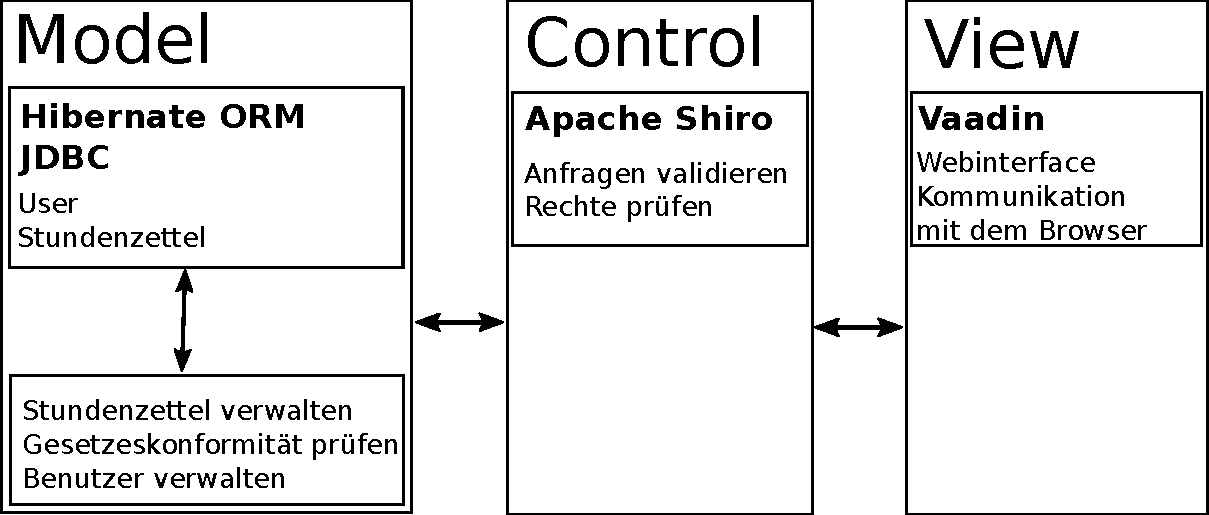
\includegraphics[width=\linewidth]{mvc.pdf}\\
\\
Die Architektur der Software basiert auf dem Model-View-Control (MVC) Modell, welches eine strikte Trennung von Daten/Logik (Model), Oberfläche (View) und Steuerung (Control) vorsieht.
Dies verbessert zum einen die Wartbarkeit und vereinfacht den Austausch einzelner Module, vor allem der Oberfläche.
\begin{itemize}
	\item \textbf{Model:}
		Das Model enthält die \emph{Benutzer*} und \emph{Stundenzettel}.
		Es enthält die Funktionalität um \emph{Benutzer*} und Stundenzettel zu verwalten.
		Außerdem prüft es, ob die \emph{Stundenzettel} den gesetzlichen Regelungen entsprechen und leitet sonst entsprechende Maßnahmen ein.
	\item \textbf{View:}
		Das View zeigt dem \emph{Benutzer*} alle Funktionalitäten und Informationen an, die für diesen relevant sind.
		Zudem nimmt es Befehle desselbigen entgegen.
		Es ist die Schnittstelle über die alle Interaktion mit dem \emph{Benutzer*} passiert.
	\item \textbf{Control:}
		Das Control prüft alle Anfragen die es vom View bekommt auf Korrektheit.
		Zudem prüft es ob der entsprechende \emph{Benutzer*} die nötigen Rechte für die Anfrage hat.
		Dann leitet es die Anfrage gegebenenfalls an das Model weiter.
\end{itemize}

%\section{Systemmodelle}
\newpage
\subsection{Anwendungsfalldiagramm}
Das System ist in die Benutzer*gruppe Benutzer*, Betreuer* und Admin* unterteilt. Folgendes Use-Case-Diagramm beschreibt die Interaktionsmöglichkeiten der einzelnen Benutzer*gruppe mit dem Server:
\begin{itemize}
	\item Mit dem Accounts Verwalten kann der Admin* neuen Benutzer* anlegen, Account abändern, Rechte vergeben oder löschen.
	\item Mit Komponente Login können Benutzer* sich anmelden bzw. abmelden.
	\item Eine Benutzer* kann neue Zeiterfassung starten. Nachträgliche Erfassung, Bearbeitung oder Korrektur ist möglich. Er darf seine eigene erfasste Zeiten und Stundenzettel ansehen. Er kann Warnungen und Erinnerungen lesen. Er druckt sein Stundenzettel aus, unterschreibt und gibt es bei seinem Betreuer* ab.
	\item Ein Betreuer* darf die Erfasste Zeiten, Stundenzettel, und Nachrichten von allen seinen zugewiesenen Benutzern* ansehen. Er kontrolliert Stundenzettel von seinen Benutzern* und gibt die Status weiter an den Admin*.
	\item Der Admin* darf alles ansehen. Außderdem sammelt er noch alle Stundenzettel ein.
\end{itemize}


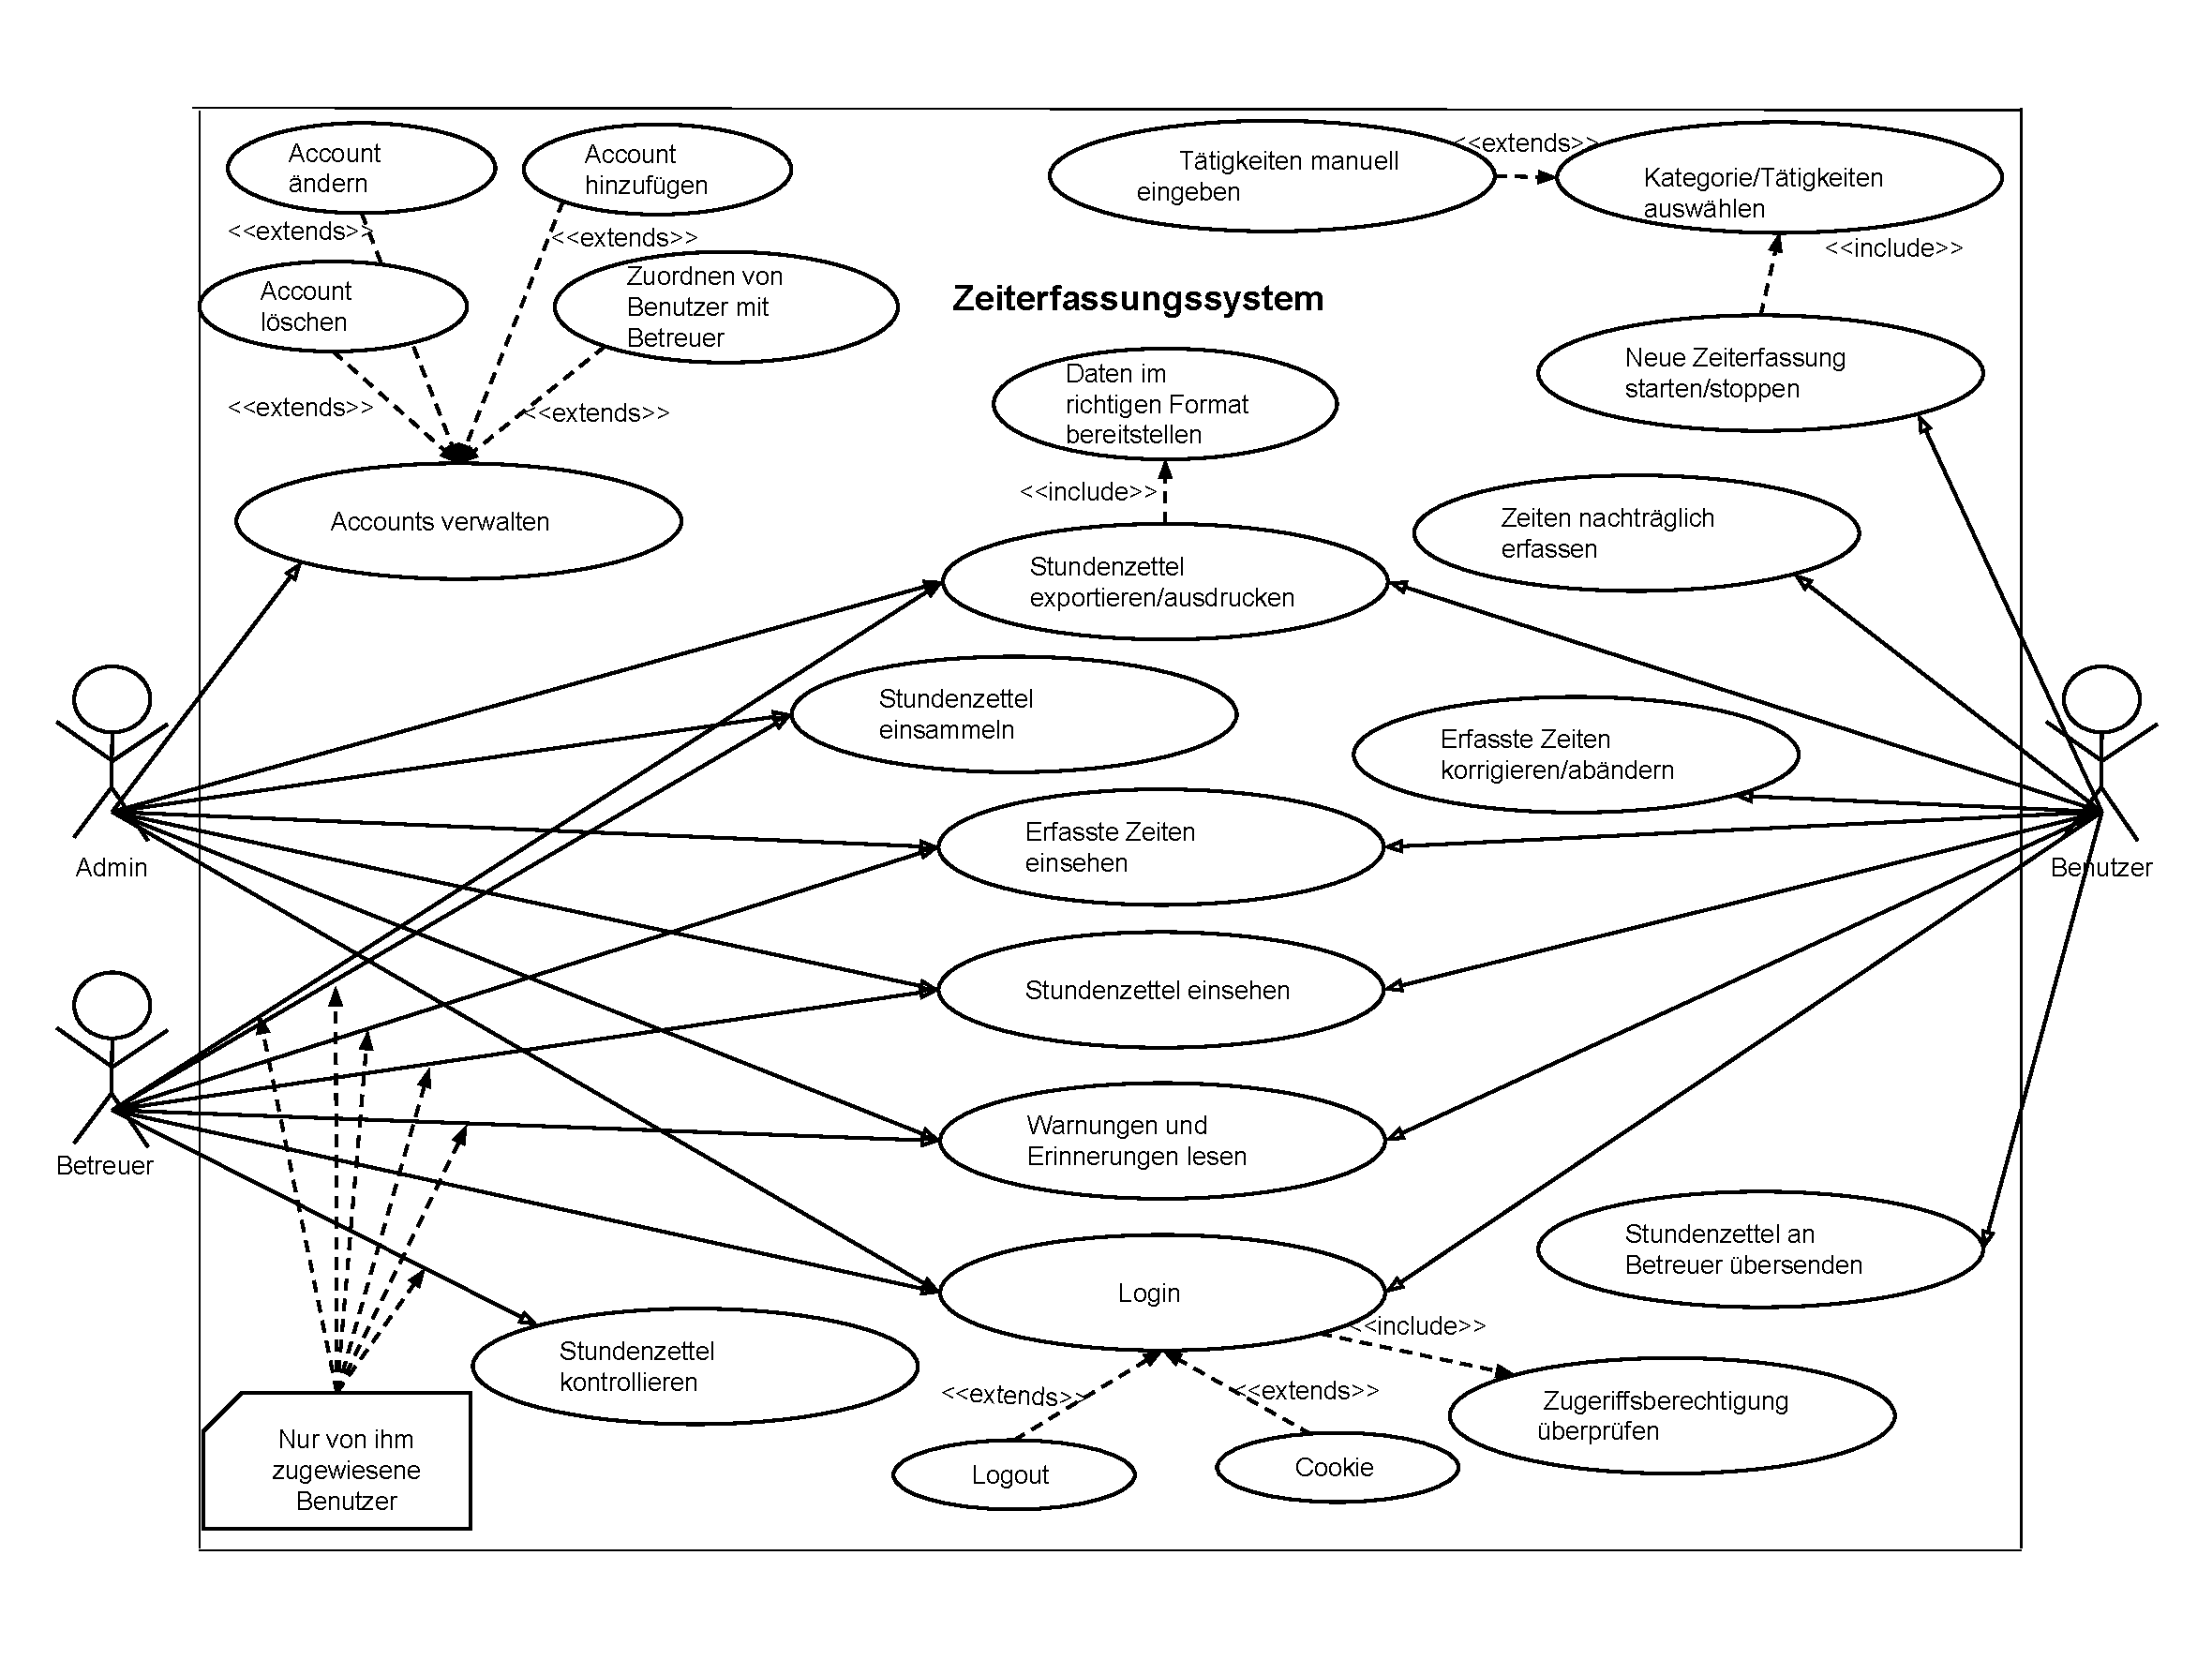
\includegraphics[width=\linewidth]{Anwendungsfalldiagramm.pdf}\\

\section{Systemdesign}

\subsection{Login}
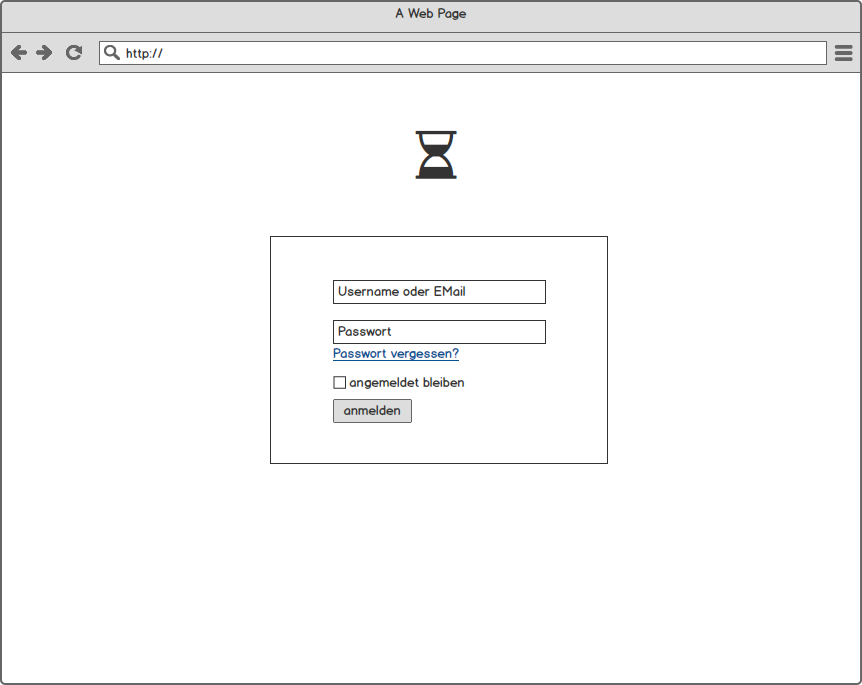
\includegraphics[width=\linewidth]{UI/Login/Login.png}

\newpage
\subsection{Benutzer*}

\textbf{\\Neue Zeiterfassung}\\
\\
Das ist die Hauptseite vom \emph{Benutzer*}, wo er direkt nach einer erfolgreichen Anmeldung oder durch Drücken auf die Schaltfläche "neue Zeiterfassung" landet. \\
Um eine neue Zeiterfassung zu starten, wählt der \emph{Benutzer*} eine Kategorie und eine Tätigkeit aus, anschließend drückt er auf Start Button. Der \emph{Benutzer*} kann die Zeiterfassung über das Stop Button beenden.\\
\\
\\
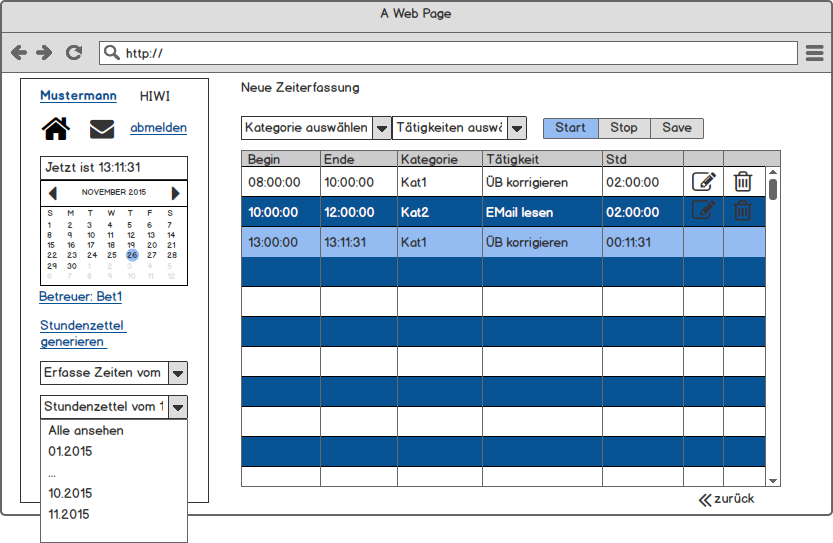
\includegraphics[width=\linewidth]{UI/Benutzer/Zeiterfassung.png}


\newpage
\textbf{\\Erfasste Zeiten bearbeiten}\\
\\
Das ist die Seite fürs Editieren der erfassten Zeiten vom \emph{Benutzer*}.
Man kann entweder direkt von der Seite "Neue Zeiterfassung" über das Edit Button 
\includegraphics[scale=.2]{UI/Button/Edit.png} oder durch auswählen vom Datum auf der Kalenderübersicht auf der linken Seite auf diese Seite landen. Nur die erfassten Zeiten, die noch nicht an den Betreuer abgegeben sind, könnten editiert werden.\\
Der \emph{Benutzer*} klickt in das Textfeld, wo er eine Änderung tätigen will, und ändert die dort eingetragene Daten. Anschließend klickt er auf das Save Button
\includegraphics[scale=.2]{UI/Button/Save.png}, um die Änderungen zu bestätigen.\\
\\
\\
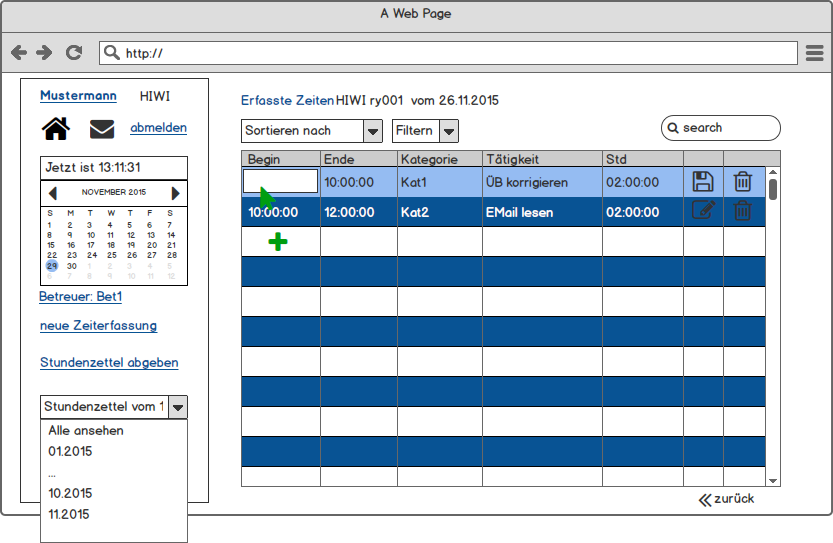
\includegraphics[width=\linewidth]{UI/Benutzer/Editieren.png}





\newpage
\textbf{\\Nachricht Interface vom Benutzer*}\\
\\
Die Nachrichten(Warnungen und Erinnerungen) sieht der \emph{Benutzer*}, indem er auf Nachricht Button

\includegraphics[scale=.8]{UI/Button/Nachricht.png} drückt.\\
Die Anzahl der Nachrichten erscheint in dem kleinen Kreis rechtsoben auf dem Button.\\
\\
\\
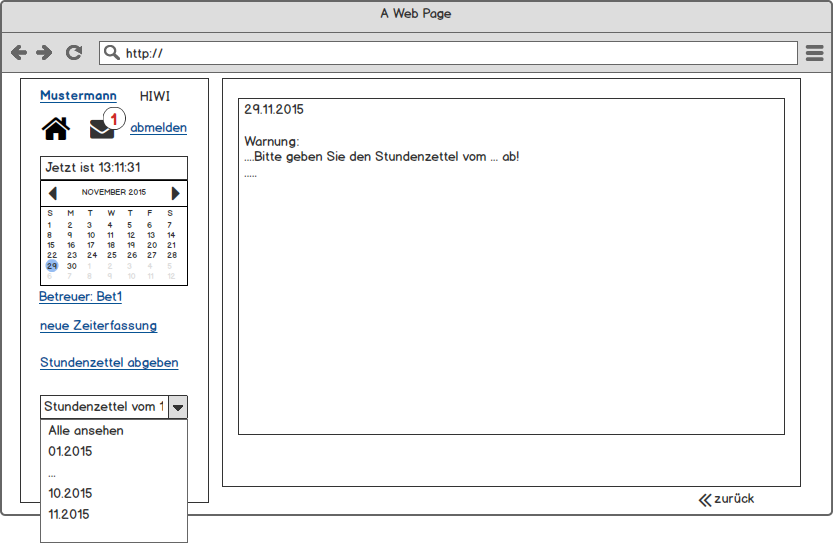
\includegraphics[width=\linewidth]{UI/Benutzer/Nachricht.png}

\newpage
\subsection{Betreuer}
\textbf{\\Hauptseite vom Betreuer*}\\
\\
Nach der erfolgreichen Anmeldung befindet sich der \emph{Betreuer*} auf dieser Seite.\\
Alle ihm zugewiesenen \emph{Benutzer*} werden samt deren Informationen und Daten angezeigt.\\
Der \emph{Betreuer*} kann hier die schon abgegebenen \emph{Stundenzettel} aufrufen, kontrollieren und ausdrucken.\\
Wenn der \emph{Stundenzettel} korrekt ist, drückt der \emph{Betreuer*} auf "Geprüft". Danach wird der \emph{Administrator} drüber informiert.\\
Wenn der \emph{Stundenzettel} nicht korrekt ist, drückt der \emph{Betreuer*} auf "Nicht OK". Dann wird ein Textfeld erscheinen, in dem der \emph{Betreuer*} die Gründe der Ablehnung schreiben kann.\\
\\
\\
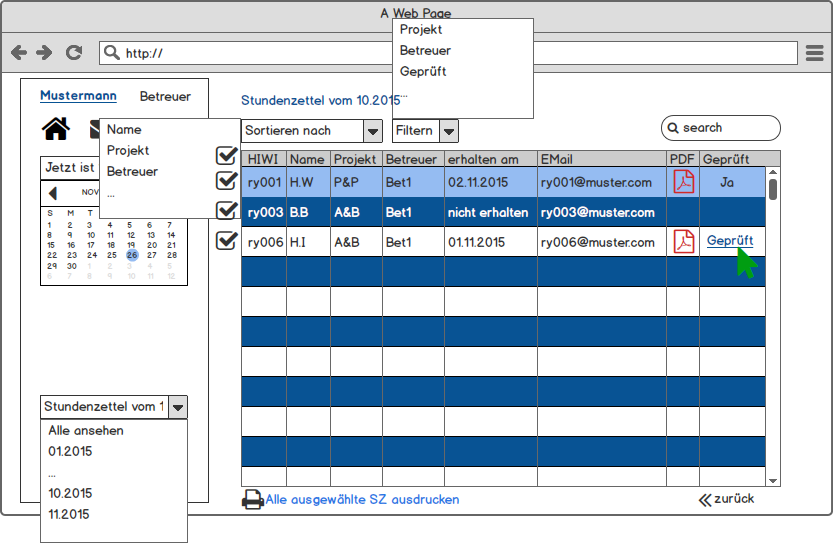
\includegraphics[width=\linewidth]{UI/Betreuer/Hauptseite.png}

\newpage
\textbf{\\Nachricht Interface vom Betreuer*}\\
\\
Auf der Nachrichtenseite wird der \emph{Betreuer*} über Erinnerungen/Warnungen an allen ihm zugewiesenen \emph{Benutzern*} und Abgabe von \emph{Stundenzettel} informiert.\\
Hier kann der \emph{Betreuer*} direkt die \emph{Stundenzettel} aufrufen, kontrollieren und Kommentar dazu schreiben.\\
\\
\\
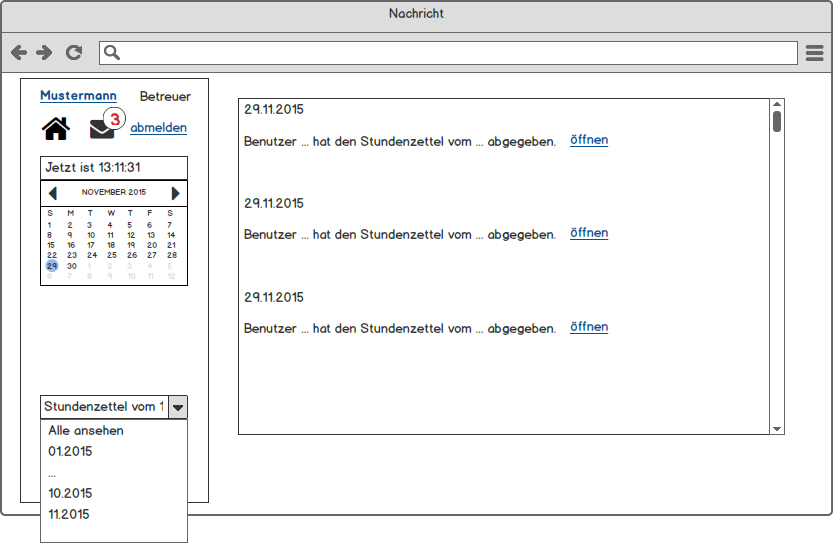
\includegraphics[width=\linewidth]{UI/Betreuer/Nachricht.png}

\newpage
\subsection{Administrator*}
\textbf{\\Hauptseite vom Administrator*}\\
\\
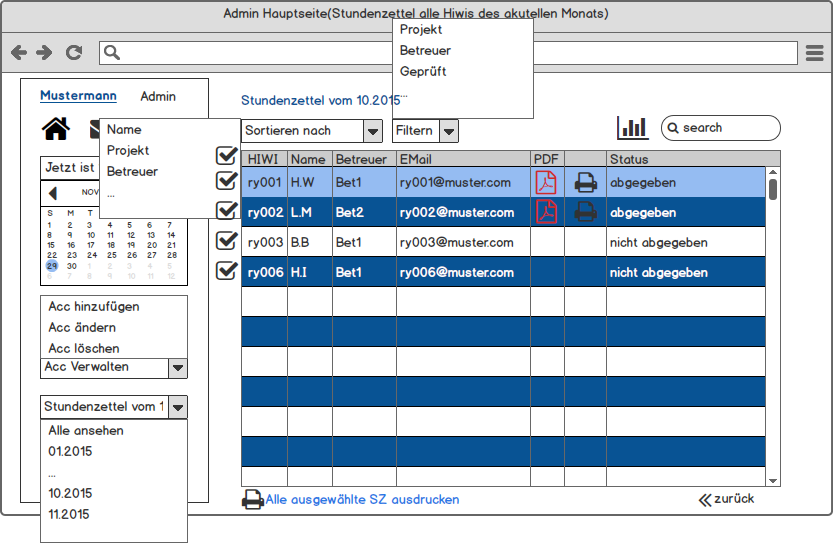
\includegraphics[width=\linewidth]{UI/Admin/Hauptseite.png}
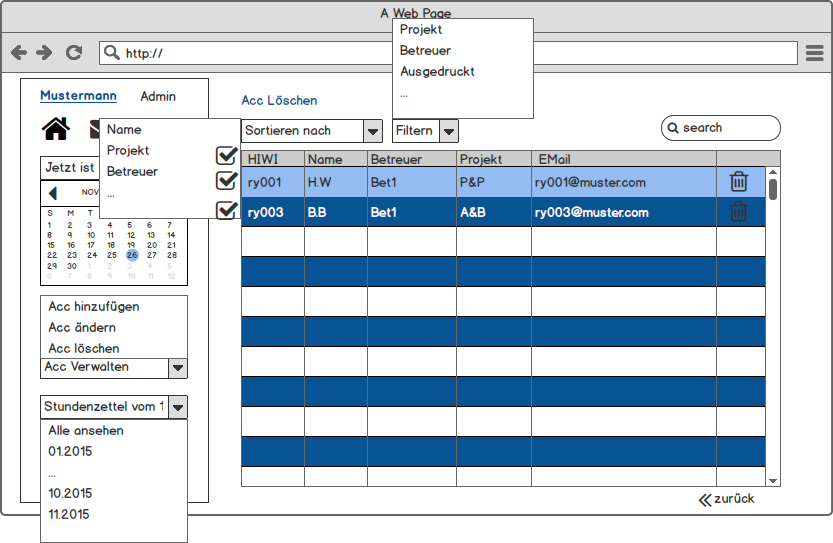
\includegraphics[width=\linewidth]{UI/Admin/Accounts/Ubersicht.png}
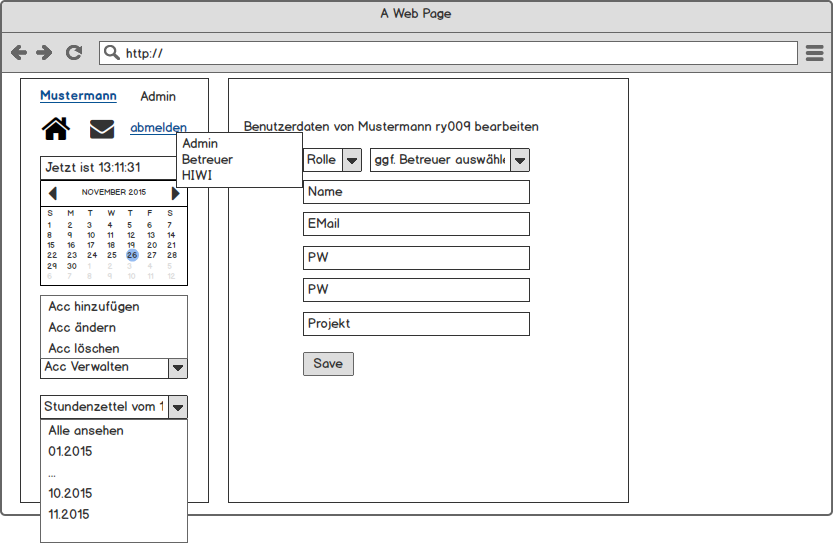
\includegraphics[width=\linewidth]{UI/Admin/Accounts/Bearbeiten.png}

\section{Glossar}
\begin{description}
	\item[Administrator*] Der \emph{Administrator*}. Höchste Entität, besitzt Rechte zum modizieren von angelegten \emph{Benutzern*}.
	               Erhält ebenfalls die \emph{abgegebenen Stundenzettel}.

	\item[ArbZG] Das deutsche Arbeitszeitgesetz

	\item[Betreuer*] Betreut mehrere \emph{Benutzer*} und kann deren \emph{Stundenzettel} einsehen.

	\item[Heatmap] Eine \emph{Heatmap} ist ein Diagramm zur Visualisierung von Daten, deren abhängige Werte einer zweidimensionalen Definitionsmenge als Farben repräsentiert werden.  \emph{(Zitat Wikipedia)}

	\item[JDBC] Eine Bibliothek um eine Vielzahl an Datenbanken nutzen zu können (z.B. MySQL oder PostgreSQL)

	\item[Kategorie] In welche \emph{Kategorie} die \emph{Tätigkeit} fällt. Zum Beispiel an welchem Projekt gearbeitet wurde

	\item[Session cookie] Eine Information die im Browser des \emph{Benutzers*} hinterlegt wird um ihn zu identifizieren, damit er nicht bei jeder Aktion sein Passwort neu eingeben muss.

	\item[Stundenzettel] Formular auf dem die geleisteten Stunden mit \emph{Tätigkeit} vermerkt werden.

	\item[Team] Gruppe von \emph{Benutzern*} die von einem \emph{Betreuer*} geleitet werden.

	\item[*] Der * bei \emph{Benutzer*} (und auch \emph{Betreuer*} und \emph{Administrator*}) deutet an, dass die Rolle von Personen jeden Geschlechts eingenommen werden kann, nicht nur von Personen die sich mit er/sein (oder sie/ihr) Pronomen identifizieren.

\end{description}


\end{document}
